
\chapter{Basic concepts in estimation}
\label{chap:theory}

An estimation problem in statistics may have many potential solutions. To
separate useful estimation strategies from approaches that are less feasible,
criteria have to be defined by which different estimators can be evaluated and
compared. In this chapter we first review a number of basic criteria typically
used in classic statistics. We then discuss additional criteria that are
important in the context of robust statistics. Our discussion in this chapter
is conceptual in nature; it is supposed to establish a theoretical basis for
the specific robust estimators that are discussed in the subsequent chapters
from an applied perspective.

\section{Classical properties of estimators}

The goal of statistical estimation is to obtain a reasonable value for the
unknown \emph{paramater} of a statistical model, based on data whose properties
are assumed to be consistent with the suggested model. Let $\mathcal{X}^{(n)} =
\{X_1, \dots, X_n\}$ be a set of $n$ random variables $X_1, \ldots, X_n$ that
have a joint probability distribution $P_{\boldsymbol\theta}^{(n)}$ depending
on the unknown parameter $\boldsymbol\theta$. Note that, depending on context,
$\boldsymbol\theta$ may be scalar, or it may be a vector of multiple
parameters, that is $\boldsymbol\theta = (\theta_1, \dots, \theta_p)^t$. For
simplicity, we consider here that the observations $X_i$ are univariate.
However, the concepts introduced hereafter may be (quite easily) generalized in
the case of multivariate observations $\stvec{X}_i$, that is, in the case
$\stvec{X}_i$ is a vector of random variables
($\stvec{X}_i=(X_{i1},\ldots,X_{ik})^t$).

Since $\boldsymbol\theta$ is unknown, this actually leads to assume that the
joint distribution of the random variables $X_i$, $i=1, \dots, n$, belongs to
the (parametric) \emph{statistical model} $\mathcal{P}^{(n)} =
\{P_{\boldsymbol\theta}^{(n)} | \boldsymbol\theta \in \boldsymbol\Theta\}$,
where $\boldsymbol\Theta$ is the set of possible values of $\boldsymbol\theta$.
The goal is to estimate $\boldsymbol\theta \in \boldsymbol\Theta$ based on a
realization of $\mathcal{X}^{(n)}$. In general, we will consider the case in
which the statistical model $\mathcal{P}^{(n)}$ conforms to simple random
sampling (\stsc{SRS}), that is, a situation in which the random variables $X_1,
\dots, X_n$ are independent and identically distributed (i.i.d.). In this
situation, each $X_i$ independently follows a common probability distribution
$P_{\boldsymbol\theta}$, which can be characterized by the distribution
function $F_{\boldsymbol\theta}(\stvec{x}) = \Pr(X_i \leq x)$ (or simply $F$
when there is no risk of confusion about the parameter we have to estimate).

An \emph{\Index{estimator}} of $\boldsymbol\theta$ can then be defined as
follows: An \Index{estimator} of the parameter $\boldsymbol\theta$ is any
statistic $\sthat{\boldsymbol\theta} =
\sthat{\boldsymbol\theta}(\mathcal{X}^{(n)})$ taking its value in
$\boldsymbol\Theta$.

The value of $\sthat{\boldsymbol\theta}$ provided by a particular realization
$x_1,\ldots,x_n$ of the random variables $X_1, \dots, X_n$ is called an
\emph{\Index{estimate}} of $\boldsymbol\theta$. Note that, for simplicity, we
will often use the notation $x_i$ ($i \in \{1, \dots, n\}$) to designate the
$i$th random observation as well as a realization of it (i.e., a specific
value); the context will always clearly indicate if we have to consider $x_i$
as a random variable or as a particular value.

The definition above contains no indication of the quality of an estimator; any
statistic $\sthat{\boldsymbol\theta}$ that provides a value in
$\boldsymbol\Theta$ is a valid estimator. To narrow down the set of estimators
to estimators that can be considered useful we need quality criteria. Classic
quality criteria are unbiasedness, efficiency, and consistency.

\subsection{Unbiasedness}
\Index[unbiasedness]{}

From a good estimator one may expect that, on average, it gives the “correct”
answer. Let us denote by
$E_{\boldsymbol\theta}(\sthat{\boldsymbol\theta}(\mathcal{X}^{(n)}))$ the
expectation of statistic $\sthat{\boldsymbol\theta}(\mathcal{X}^{(n)})$ when
$\mathcal{X}^{(n)} \sim P_{\boldsymbol\theta}^{(n)}$. Think of
$E_{\boldsymbol\theta}$ as the average value we would obtain for
$\sthat{\boldsymbol\theta}$ from a large number of repeated realizations of
$\mathcal{X}^{(n)}$, given that for each repetition $\mathcal{X}^{(n)}$ follows
distribution $P_{\boldsymbol\theta}^{(n)}$ (as, for example, in repeated random
sampling from the same population).

Unbiasedness can then be defined as follows:
The estimator $\sthat{\boldsymbol\theta} = \sthat{\boldsymbol\theta} 
(\mathcal{X}^{(n)})$ is called unbiased if
\[
    E_{\boldsymbol\theta}(\sthat{\boldsymbol\theta}) = \boldsymbol\theta
    \qquad
    \text{for all $\boldsymbol\theta \in \boldsymbol\Theta$ and all $n$}.
\]

That is, no matter the sample size $n$, estimator $\sthat{\boldsymbol\theta}$
will, on average across a large number of repeated samples, provide the correct
value of $\boldsymbol\theta$ (given that our assumptions about the joint distribution of
$\mathcal{X}^{(n)}$ are correct, such as, e.g., independent sampling of
observations). The difference
\[
    B_{\boldsymbol\theta}(\sthat{\boldsymbol\theta}) 
        = E_{\boldsymbol\theta}(\sthat{\boldsymbol\theta}) - \boldsymbol\theta
\]
is called the \emph{\Index{bias}} of estimator $\sthat{\boldsymbol\theta}$.
The absence of bias indicates that the sampling distribution of
$\sthat{\boldsymbol\theta}$ has a mean that coincides with the value of the
parameter of interest.

Zero bias is often difficult to achieve in small samples. Therefore, another
useful criterion is \emph{asymptotic unbiasedness}: The estimator
$\sthat{\boldsymbol\theta} = \sthat{\boldsymbol\theta}(\mathcal{X}^{(n)})$ is
called asymptotically unbiased if
\[
    \lim_{n \rightarrow \infty} E_{\boldsymbol\theta}(\sthat{\boldsymbol\theta}) = \boldsymbol\theta
    \qquad
    \text{for all $\boldsymbol\theta \in \boldsymbol\Theta$}.
\]

That is, an estimator is asymptotically unbiased if the bias vanishes with 
increasing sample size. An important question in this context is, of course, how 
fast the bias vanishes (or how large the sample size has to be for the bias to be 
negligible).

\subsection{Efficiency}

For a specific estimation problem, several (asymptotically) unbiased estimators
may exist. To choose the best among them we need further information about the
performance of the different estimators. Furthermore, there may also be
situations in which a biased estimator is to be preferred over an unbiased
estimator. A key aspect in this regard is the \emph{\Index{efficiency}} of an
estimator. Efficiency has to do with how spread out about $\boldsymbol\theta$
the sampling distribution of the estimator is. The smaller the dispersion of
estimator $\sthat{\boldsymbol\theta}$ around the true value
$\boldsymbol\theta$ in repeated samples, the more “efficient” (or precise) is
the estimator.

\paragraph{Mean squared error}

First consider the case of a \emph{scalar} parameter $\theta$. The
precision of estimator $\sthat{\theta}$ can be measured by its
\emph{\Index{mean squared error}} (\stsc{MSE}):
\[
    \stsc{MSE}_{\theta}(\sthat{\theta}) 
    = E_{\theta} \left((\sthat{\theta} - \theta)^2\right).
\]
A small mean squared error for $\sthat{\theta}$ means that the sampling
distribution of $\sthat{\theta}$ is well concentrated around the exact value
of the parameter to estimate and hence that the estimator $\sthat{\theta}$
has a good precision.

It is easy to show that
\[
    \stsc{MSE}_{\theta}(\sthat{\theta})
    = \mathrm{Var}_{\theta}(\sthat{\theta}) 
      + \left(B_{\theta}(\sthat{\theta})\right)^2.
\]
That is, the mean squared error of an estimator can be decomposed into its
variance and its squared bias. Hence, if $\sthat{\theta}$ is unbiased,
$\stsc{MSE}_{\theta}(\sthat{\theta})$ is simply equal to
$\mathrm{Var}_{\theta}(\sthat{\theta})$.

\paragraph{Relative efficiency}

An estimator $\sthat{\theta}_A$ of $\theta$ is more precise---we will say
\emph{more efficient}---than another estimator $\sthat{\theta}_B$ if
\[
    \stsc{MSE}_{\theta}(\sthat{\theta}_A) \leq 
    \stsc{MSE}_{\theta}(\sthat{\theta}_B)
    \qquad\text{for all $\theta \in \Theta$}
\]
and
\[
    \stsc{MSE}_{\theta}(\sthat{\theta}_A) < 
    \stsc{MSE}_{\theta}(\sthat{\theta}_B)
    \qquad\text{for at least one $\theta \in \Theta$}.
\]


In general, we consider the “large-sample” sampling distributions of
asymptotically unbiased estimators. If, for large $n$, the estimators
$\sthat{\theta}_A$ and $\sthat{\theta}_B$ are approximately
$\mathcal{N}(\theta, \textrm{Var}(\sthat{\theta}_A))$ and
$\mathcal{N}(\theta, \textrm{Var}(\sthat{\theta}_B))$, respectively, we
define the \emph{\Index{asymptotic relative efficiency}} (\stsc{ARE}) of
$\sthat{\theta}_B$ with respect to $\sthat{\theta}_A$ as the ratio
\[
    \stsc{ARE}_{\theta}(\sthat{\theta}_B,\sthat{\theta}_A) 
    = \frac{ \textrm{Var}(\sthat{\theta}_A)}{\textrm{Var}(\sthat{\theta}_B)}
\]
(see \citealp{Serfling1980}). If $\sthat{\theta}_B$ is (asymptotically) less
efficient than $\sthat{\theta}_A$, then
\[
    \stsc{ARE}_{\theta}(\sthat{\theta}_B,\sthat{\theta}_A) \leq 1
\]
for all $\theta \in \Theta$, with strict inequality holding for at least some
value of $\theta$.


\paragraph{Efficiency of the maximum likelihood estimator}

Let us consider the case in which the random variables $X_1, \ldots, X_n$ of
the sample ${\cal X}^{(n)}$ are i.i.d.\ with a common distribution function
$F_{\theta}$ and a common density function $f_{\theta}$ that satisfies some
differentiability conditions with respect to $\theta$. Suppose also that the
\emph{\Index{Fisher information}}
\[
    \mathcal{I}\left(F_{\theta}\right) =
        E_{\theta}\left(\left(\frac{\partial}{\partial\theta}
        \log f_{\theta}(X)\right)^2\right)
\] 
is strictly positive and finite. Then it follows that
\begin{enumerate}
    \item[(i)] for large $n$, the maximum likelihood estimator
    $\sthat{\theta}_{\stsc{ML}}$ of $\theta$ is approximately distributed as
    $\mathcal{N}\left(\theta, (n \mathcal{I}(F_{\theta}))^{-1}\right)$
    
    \item[(ii)] for a wide class of estimators $\sthat{\theta}$ that are
    approximately distributed as $\mathcal{N}(\theta, V)$, a \emph{lower
    bound} to $V$ is $(n \mathcal{I}(F_{\theta}))^{-1}$
\end{enumerate}
(see \citealp{LehmannCasella1988}). In this situation,
%
\begin{equation}\label{eq:ARE_vsML}
    \stsc{ARE}_{\theta}(\sthat{\theta}, \sthat{\theta}_{\stsc{ML}})
     = \frac{(n \mathcal{I}(F_{\theta}))^{-1}}{V} \leq 1
\end{equation}
%
for all $\theta \in \Theta$, making $\sthat{\theta}_{\stsc{ML}}$ the most
(asymptotically) efficient among the given class of estimators
$\sthat{\theta}$. Note, however, as will be discussed later, that
(\ref{eq:ARE_vsML}) does not necessarily make $\sthat{\theta}_{\stsc{ML}}$ the
estimator of choice, when certain other considerations are taken into account.


\paragraph{Notation in the multidimensional case}

If $\boldsymbol\theta = (\theta_1, \dots, \theta_p)^t$ is a vector of parameters
we define the \emph{\Index[mean squared error!matrix]{mean squared error matrix}}
of the estimator $\sthat{\boldsymbol\theta}$ as follows:
\[
    \stsc{MSE}_{\boldsymbol\theta}(\sthat{\boldsymbol\theta})
    = E_{\boldsymbol\theta}\left((\sthat{\boldsymbol\theta} - \boldsymbol\theta)
                                 (\sthat{\boldsymbol\theta} - \boldsymbol\theta)^t
                           \right).
\]
If $\sthat{\boldsymbol\theta}$ is unbiased, the mean squared error matrix simply
coincides with the covariance matrix of the estimator.

If, for large $n$, the $p$-variate estimators $\sthat{\boldsymbol\theta}_A$ and
$\sthat{\boldsymbol\theta}_B$ are approximately normally distributed with mean
$\boldsymbol\theta$ and nonsingular covariance matrices $\boldsymbol\Sigma_A$ and
$\boldsymbol\Sigma_B$, respectively, it is usual to define the 
\emph{\Index{asymptotic relative efficiency}} (\stsc{ARE}) of
$\sthat{\boldsymbol\theta}_B$ with respect to $\sthat{\boldsymbol\theta}_A$ as
the ratio of the \emph{generalized variances} (determinants of the covariance
matrices), raised to the power $1/p$, that is
\[
    \stsc{ARE}_{\boldsymbol\theta}(\sthat{\boldsymbol\theta}_B, \sthat{\boldsymbol\theta}_A)
    = \left(\frac{ \det(\boldsymbol\Sigma_A)}{\det(\boldsymbol\Sigma_B)}\right)^{1/p}.
\]
If $\stsc{ARE}_{\boldsymbol\theta}(\sthat{\boldsymbol\theta}_B,
\sthat{\boldsymbol\theta}_A) \leq 1$ for all $\boldsymbol\theta \in
\boldsymbol\Theta$, with strict inequality holding for at least some value
$\boldsymbol\theta$, estimator $\sthat{\boldsymbol\theta}_B$ is
(asymptotically) less efficient than estimator $\sthat{\boldsymbol\theta}_A$.

Here again the maximum likelihood estimator $\sthat{\boldsymbol\theta}_\stsc{ML}$ of
$\boldsymbol\theta$ appears as the most (asymptotically) efficient estimator among a
wide class of (asymptotically) unbiased estimators $\sthat{\boldsymbol\theta}$ of
$\boldsymbol\theta$. Moreover, for large $n$,
\[
    \sthat{\boldsymbol\theta}_\stsc{ML} \approx 
    \mathcal{N}\left(\boldsymbol\theta, (n \stmat{I}(F_{\boldsymbol\theta}))^{-1}\right)
\]
where “$\approx$” stands for “is approximately distributed as” and
$\stmat{I}(F_{\boldsymbol\theta})$ is the $p\times p$ Fisher information matrix
with its elements defined as
\[
    \mathcal{I}_{ij}\left(F_{\boldsymbol\theta}\right) =
    E_{\boldsymbol\theta}\left(
    \frac{\partial}{\partial\theta_i}\log f_{\boldsymbol\theta}(X) \times 
    \frac{\partial}{\partial \theta_j}\log f_{\boldsymbol\theta}(X)
    \right).
\] 


\subsection{Consistency}
\Index[consistency]{}

High efficiency and (asymptotic) unbiasedness are desired properties for an
estimator. But other properties are still required if we want the estimator to
provide valid statistical inference for $\boldsymbol\theta$.

The sampling distribution of $\sthat{\boldsymbol\theta}$ generally depends on
the size $n$ of the sample, e.g. via its mean, its variance and (or) other
characteristics. How does the distribution of $\sthat{\boldsymbol\theta}$
evolve when $n$ increases? This question will first lead us to the properties
of \emph{(asymptotic) consistency} ---\emph{convergence in probability}--- and
\emph{Fisher consistency}. We will then consider the concept of
\emph{convergence in distribution}.

\paragraph{(Asymptotic) consistency: Convergence in probability}
\Index[convergence!in probability]{}
\Index[consistency!asymptotic]{}

An estimator $\sthat{\boldsymbol\theta} =
\sthat{\boldsymbol\theta}(\mathcal{X}^{(n)})$ is \emph{consistent} or
\emph{asymptotic consistent} if, for $n \rightarrow \infty$,
$\sthat{\boldsymbol\theta}$ \emph{converges in probability} to
$\boldsymbol\theta$. That is, for any $\epsilon > 0$ and for all
$\boldsymbol\theta \in \boldsymbol\Theta$:
\begin{equation}
    \lim_{n \rightarrow \infty} P_{\boldsymbol\theta}^{(n)} \left(
        \Vert\sthat{\boldsymbol\theta} - \boldsymbol\theta \Vert \leq \epsilon
        \right) = 1. \label{eq:consistency}
\end{equation}

This type of convergence means that, when the sample size grows, the
probability that the estimator $\sthat{\boldsymbol\theta}$ takes a value
arbitrarily close to the exact value of the parameter and, consequently,
provides a “good” estimate of the parameter $\boldsymbol\theta$, grows to 1.

In other terms, a consistent estimator $\sthat{\boldsymbol\theta}$ of
$\boldsymbol\theta$ is an estimator that becomes more and more precise when the
number of observations increases. It also means that the sampling distribution
of $\sthat{\boldsymbol\theta}$ becomes more and more concentrated around the
true value of the parameter being estimated. This property of consistency is of
course a highly desirable property for an estimator.

\paragraph{Convergence in quadratic mean}
\Index[convergence!in quadratic mean]{}

Another type of convergence is closely related to the notion of consistency:
the \emph{convergence in quadratic mean}. For simplicity, consider the case of
a scalar parameter $\theta$: $\sthat{\theta}=\sthat{\theta}({\cal X}^{(n)})$
converges in quadratic mean to $\theta$ if
\[
    \stsc{MSE}_{\theta}(\sthat{\theta})=E_{\theta}\left((\sthat{\theta}-\theta)^2\right) 
    \stackrel{n \rightarrow \infty}{\longrightarrow} 0.
\]

Since $\stsc{MSE}_{\theta}(\sthat{\theta})={\rm Var}_{\theta}(\sthat{\theta}) +
\left(B_{\theta}(\sthat{\theta})\right)^2$, it is clear that, if
$\sthat{\theta}$ is asymptotically unbiased and has a variance that tends to
zero when $n$ tends to infinity, then $\sthat{\theta}$ converges to $\theta$ in
quadratic mean. Moreover, it is quite easy to prove that the convergence in
quadratic mean implies the convergence in probability. This result is intuitive
since $\stsc{MSE}_{\theta}(\sthat{\theta})$ is nothing but a measure of the
dispersion of the sampling distribution of $\sthat{\theta}$ around the exact
value of the parameter to estimate.

In practice, it is often easier to establish the consistency of
$\sthat{\theta}$ by verifying that $\sthat{\theta}$ converges in quadratic mean
to $\theta$ instead of considering directly the equality (\ref{eq:consistency}).

\paragraph{Fisher consistency}
\Index[consistency!Fisher]{}

In statistics, \emph{Fisher consistency} is another desirable property of an
estimator asserting that if the estimator were calculated using the entire
population rather than a sample, the true value of the estimated parameter
would be obtained (\citealp{fisher:1922}).

Suppose we have a statistical sample ${\cal X}^{(n)}=\{X_1,\ldots,X_n\}$ where
each $X_i$ has a distribution characterized by the cumulative distribution
$F_{\boldsymbol\theta}$ which depends on an unknown parameter
$\boldsymbol\theta$. If the estimator
$\sthat{\boldsymbol\theta}=\sthat{\boldsymbol\theta}({\cal X}^{(n)})$ can be
represented as a \emph{functional} of the empirical distribution
function\footnote{The empirical distribution function $F^{(n)}$ is the
distribution function associated with the discrete probability distribution
allocating a probability mass of $1/n$ at each observation $X_i$,
$i=1,\ldots,n$, of the sample ${\cal X}^{(n)}$.} $F^{(n)}$, that is,
\[
    \sthat{\boldsymbol\theta}=\stvec{T}(F^{(n)}),
\] 
$\sthat{\boldsymbol\theta}$ is said to be \emph{Fisher consistent} if
\[
    \stvec{T}(F_{\boldsymbol\theta})=\boldsymbol\theta .
\]

If the strong law of large numbers can be applied, the empirical distribution
function $F^{(n)}$ converges pointwise to $F_{\boldsymbol\theta}$ when $n$
tends to infinity, allowing us to express Fisher consistency as the following
convergence property: The estimator
$\sthat{\boldsymbol\theta}=\stvec{T}(F^{(n)})$ is Fisher consistent if
\[
    \stvec{T}\left(\lim_{n\rightarrow\infty} F^{(n)}\right)=\boldsymbol\theta .
\] 

Fisher consistency and (asymptotic) consistency are distinct concepts, although
both aim to define a desirable property of an estimator. While many estimators
are consistent in both senses, neither definition encompasses the other: There
exist estimators that are (asymptotically) consistent but not Fisher consistent
and, inversely, there are estimators that are Fisher consistent but not
(asymptotically) consistent.

\subsection{Convergence in distribution}
\Index[convergence!in distribution]{}

A last type of convergence is important when we have to provide a confidence
interval for (each component of) $\boldsymbol\theta$ or to define a statistical
test to solve a testing problem for the unknown parameter $\boldsymbol\theta$:
The \emph{convergence in distribution}. Since this property concerns usually a
function of an estimator $\sthat{\boldsymbol\theta}$ of $\boldsymbol\theta$
than the estimator $\sthat{\boldsymbol\theta}$ itself, we formulate it in a
general way for a statistic $\stvec{U}^{(n)}=\stvec{U}({\cal X}^{(n)})$.

The statistic $\stvec{U}^{(n)}$ \emph{converges in distribution} to the
probability distribution ${\cal L}$ if, for $n \rightarrow \infty$, the
distribution function $F_{\stvec{U}^{(n)}}$ of $\stvec{U}^{(n)}$ converges to
the distribution function $F_{\cal L}$ associated with ${\cal L}$ in any point
of continuity of $F_{\cal L}$. That is, convergence in distribution is given if
\[
    F_{\stvec{U}^{(n)}}(\stvec{u}) \stackrel{n \rightarrow \infty}{\longrightarrow} F_{\cal L}(\stvec{u})
\] 
for any continuity point $\stvec{u}$ of the distribution function $F_{\cal L}$.

As a shorthand, we will write
\[
    \stvec{U}^{(n)} \stackrel{d}{\rightarrow} \mathcal{L}
\]
to denote convergence in distribution for $n \rightarrow \infty$. In practice, 
convergence in distribution means that, for large $n$, we may consider that
$\stvec{U}^{(n)}$ is approximately distributed as $\mathcal{L}$, that is,
\[
    \stvec{U}^{(n)} \approx \mathcal{L}.
\]

In practice, it is useful to consider an estimator $\sthat{\boldsymbol\theta}$
of $\boldsymbol\theta$ such that a certain function of
$\sthat{\boldsymbol\theta}$ converges in distribution to a well known
probability distribution ${\cal L}$ as, for example, a normal distribution, a
Student distribution, a chi-square or a Fisher distribution. Indeed it allows
to develop inference procedures for $\boldsymbol\theta$, based on
$\sthat{\boldsymbol\theta}$, that are valid when the sample size $n$ is not too
small.

\subsection{Other aspects}

Depending on context, a number of other criteria can be important. For example,
from a practical perspective, \emph{computational complexity} can be a relevant
criterion to choose between different estimators. In general, estimators that
require operations in the order of $n^2$ (that is, if the number of required
computational operations grows quadratically with the sample size) lead to
prohibitive computational costs in large samples. In many cases it is possible
to design alternative estimators (or improved computational algorithms
for a given estimator) that only require operations in the order of $\ln n$ and
are thus much more efficient (with respect to computer time) in large samples.
\alert{[Maybe expand a bit on this.]}

Furthermore, consistent estimators may differ in their \emph{rate of
convergence}, that is, in how fast the mean squared error diminishes with
growing sample size. 

If $\stsc{MSE}_{\boldsymbol\theta}(\sthat{\boldsymbol\theta})$ is of order
$n^{-\nu}$ (with $\nu > 0$ such that the mean squared error of
$\sthat{\boldsymbol\theta}$ tends to zero when $n$ tends to infinity, ensuring
the convergence of $\sthat{\boldsymbol\theta}$ in quadratic mean and, hence, in
probability), the rate of convergence of $\sthat{\boldsymbol\theta}$ is said to
be equal to $n^{\nu/2}$. This rate of convergence is actually the factor by
which we have to multiply $\sthat{\boldsymbol\theta}$ to obtain a mean squared
error that does not depend anymore on the sample size $n$. Most of estimators
in parametric models have a mean squared error of order $n^{-1}$ and,
consequently, enjoy a rate of convergence equal to $\sqrt{n}$. It is the case,
for example, for the least squares estimator of the regression coefficients
vector in the classical linear regression model. The squared root of $n$ is
certainly considered as the usual rate of convergence in the parametric
context. In the nonparametric context, we may encounter estimators whose rate
of convergence is smaller than $\sqrt{n}$. This is the case, for instance, for
a kernel estimator of a density function $f$: The kernel estimator of $f(x)$
has a mean squared error of order $n^{-4/5}$ and hence a rate of convergence
equal to $n^{2/5}$.

Naturally, an estimator with a faster rate of convergence is usually to be
preferred over an estimator with a slower rate of convergence.

Finally, an estimator should be \emph{equivariant} to transformations of data.
That is, a transformation of the data should affect the estimator
$\sthat{\boldsymbol\theta}$ in the same functional way as it affects the true
parameter $\boldsymbol\theta$. For example, let $\theta_A$ be the expected
value of variable $X_A$ and $\theta_B$ be the expected value of variable $X_B$.
If $X_B$ can be expressed as a linear combination of $X_A$, that is, $X_B = a +
b X_A$, then $\theta_B = a + b \theta_A$. In this case, also
$\sthat{\theta}_B = a + b \sthat{\theta}_A$ should hold. In other words,
whether you express your data in Dollars or in Euros, whether you express your
data in degrees Fahrenheit or degrees Celsius should only affect the scaling of
your estimator, but should not affect your results otherwise.


\section{Measures of robustness}

Intuitively, the classical approach to statistics is about defining estimators
that have desirable properties under a specified model. The goal of
robust methods, however, is to develop estimators that perform well also in the
“neighborhood” of such a model. This leads to the proposition of so called
“robust” estimators, that are, for instance, not affected too strongly or too
quickly by the presence of outliers. Although outliers are only one of
the main concerns of robust methods, we will make our first steps into
robustness theory by presenting some basic concepts for measuring the degree to
which estimators are affected by atypical observations.


\begin{stexample}
    Consider the following observations of the grades achieved by $n = 25$ students
    in fifth year of primary school (on a scale of 0 to 10):                       
    
    \begin{center}
    \begin{tabular}{rrrrrr}%
    6.00 & 6.50 & 7.00 & 7.00 & 7.00\\
    7.00 & 7.00 & 7.50 & 7.50 & 8.00\\
    8.00 & 8.00 & 8.50 & 8.50 & 8.50\\
    8.50 & 9.00 & 9.00 & 9.50 & 9.50\\
    9.50 & 9.50 & 9.50 & 9.50 & 10.00
    \end{tabular}
    \end{center}
    
    If we calculate on these data two \emph{measures of location}, the \Index{mean} and the
    \Index{median}, as well as two \emph{measures of scale}, the
    \Index{standard deviation} and the \Index{interquartile range}, the results
    are as follows:
    
\begin{stlog}
. drop _all
{\smallskip}
. matrix x = (6.00, 6.50, 7.00, 7.00, 7.00,    ///
>             7.00, 7.00, 7.50, 7.50, 8.00,    ///
>             8.00, 8.00, 8.50, 8.50, 8.50,    ///
>             8.50, 9.00, 9.00, 9.50, 9.50,    ///
>             9.50, 9.50, 9.50, 9.50, 10.00)'
{\smallskip}
. quietly svmat x
{\smallskip}
. tabstat x, statistics(mean median sd iqr)
{\smallskip}
    variable {\VBAR}      mean       p50        sd       iqr
\HLI{13}{\PLUS}\HLI{40}
          x1 {\VBAR}      8.22       8.5  1.137248       2.5
\HLI{13}{\BOTT}\HLI{40}
{\smallskip}

\end{stlog}
    
    Now, imagine the dot separating the decimals in the last observation is
    mistakenly removed, so that the last observation is coded as 1000. In this 
    case the results are the following:
    
\begin{stlog}
. replace x1 = 1000 in l
(1 real change made)
{\smallskip}
. tabstat x1, statistics(mean median sd iqr)
{\smallskip}
    variable {\VBAR}      mean       p50        sd       iqr
\HLI{13}{\PLUS}\HLI{40}
          x1 {\VBAR}     47.82       8.5  198.3737       2.5
\HLI{13}{\BOTT}\HLI{40}
{\smallskip}

\end{stlog}
    
    As is evident, the \Index{mean} and the \Index{standard deviation} strongly
    increased due to the introduction of the erroneous observation, whereas
    the \Index{median} and the \Index{interquartile range} remained unchanged.
    The example illustrates the fact that one single outlier may “break” the
    \Index{mean} and the \Index{standard deviation}, but does not affect the
    \Index{median} or the \Index{interquartile range}. Hence, these two later
    statistics can be considered as being more robust to erroneous data than
    the two first ones.

\end{stexample}

How can the degree of robustness of different statistics be quantified? How can
we compare the robustness of different estimators from various viewpoints?
These are questions we will address in the rest of this section.

In robust estimation theory it is common to consider \emph{parameters} as
\emph{functionals}. More precisely, the functional by which a
parameter\footnote{For the sake of simplicity, we will only consider here
\emph{scalar} parameters.} $T$ is defined is a rule that maps every
distribution function $F$ into a real number, that is, $T = T(F)$.\footnote{$F$
is the cumulative distribution function of a random variable $X$. Evaluated at
position $x$, the function returns the probability that the random variable
will take on a value lower than or equal to $x$, that is, $F(x) = \Pr(X \leq
x)$. In order to avoid unnecessary technical difficulties we will generally
assume in this chapter that the distribution $F$ is continuous with density
$f$. The density is the first derivative of $F$; it is nonnegative and
integrates to one.} Often, a natural \emph{estimate} $T^{(n)}$ of the parameter
$T(F)$ based on sample ${\mathcal X}^{(n)}= \{x_1, \dots, x_n\}$---where $x_1,
\dots, x_n$ are realizations of $n$ independent and identically distributed
(i.i.d.) random variables $X_1, \dots, X_n$ of distribution $F$---may be
defined as the value of the functional at the empirical distribution
$F^{(n)}$.\footnote{The empirical distribution function $F^{(n)}$ is the
distribution function associated with the discrete probability distribution
allocating a probability mass of $1/n$ at each observation $x_i$,
$i=1,\ldots,n$, of the sample ${\mathcal X}^{(n)}$.} That is, $T^{(n)} =
T(F^{(n)})$. For example, if
\[
    T(F) = \int_{-\infty}^\infty x \dif F(x) = \mu
\]
is the expected value of the distribution $F$, then
\[
    T^{(n)} = T(F^{(n)}) = \int_{-\infty}^\infty x \dif F^{(n)}(x) 
          = \frac{1}{n} \sum_{i=1}^n x_i = \mu^{(n)}
\]
is the arithmetic \Index{mean} of a sample ${\mathcal X}^{(n)}$ from $F$.
Likewise, if $T(F) = F^{-1}(0.5) = Q_{0.5}$ is the \Index{median} of the
distribution $F$, then $T^{(n)} = T(F^{(n)}) = (F^{(n)})^{-1}(0.5) =
Q_{0.5}^{(n)}$ is the empirical median of a sample ${\cal X}^{(n)}$ from $F$.

The robustness of a statistic (or estimator) $T^{(n)}$ may be analyzed in a very
intuitive way by studying how a contamination of the sample
$\mathcal{X}^{(n)}$ affects $T^{(n)}$. This empirical approach leads to the notions of
the \emph{\Index{sensitivity curve}} and the \emph{\Index[breakdown
point!finite-sample]{finite-sample breakdown point}} of $T^{(n)}$. But it is also
of great interest to consider the limiting case where $n$ tends to infinity. As
the sample size $n$ grows, the empirical distribution function $F^{(n)}$ approaches
the underlying population distribution function $F$, and the empirical measures
of robustness of the statistic $T^{(n)}$ move in a natural way to the concepts of
the \emph{\Index{influence function}} and the \emph{\Index[breakdown
point!asymptotic]{asymptotic breakdown point}} of the functional $T$.


\subsection{The sensitivity curve and the influence function}
\label{subsec:theory:IF}

\subsubsection{The sensitivity curve}
\index{subject}{sensitivity curve|(textbf}

The \textit{sensitivity curve} (\stsc{SC}) is an empirical tool to quantify the
robustness of a statistic in a given sample. Consider a data set
$\mathcal{X}^{(n)} = \{x_1, \dots, x_n\}$ and the statistic $T^{(n)} =
T^{(n)}(x_1, \dots, x_n) = T(F^{(n)})$. To study the impact of a potential
outlier on this statistic, we may analyze the change in the value of the
statistic once we add an extra data point $x$, where $x$ is varied between
$-\infty$ an $+\infty$. Hence, the \emph{(standardized) sensitivity curve} of
statistic $T^{(n)}$ for the sample $\mathcal{X}^{(n)}$ is defined as
\[
    \stsc{SC}(x; T^{(n)}, \mathcal{X}^{(n)}) = 
    \frac{T^{(n+1)}(x_1, \dots, x_n, x) - T^{(n)}(x_1, \dots, x_n)}{\frac{1}{n+1}}\ \cdot
\]
That is, for each value of $x$ we compare the statistic in the “contaminated”
sample to its value in the original sample, and rescale the difference by
dividing the difference by $1/(n+1)$, the proportion of contamination.

\begin{stexample}
Consider a data set $\mathcal{X}^{(n)}$ of $n=20$ (rounded) random numbers from a
$\mathcal{N}(0,1)$ (standard normal) distribution:
\begin{center}\begin{tabular}{*{10}{D{.}{.}{2.2}}}
    -0.49 &      0.14 &      1.54 &      0.63 &     -0.87 &     -0.86 &      1.65 &     -0.55 &      0.91 &     -0.03 \\
    -0.61 &      0.22 &     -1.61 &      0.15 &      0.36 &      1.96 &      1.04 &      0.24 &     -0.45 &      0.98
\end{tabular}\end{center}

Figure \ref{fig:theory:SClocation} shows the standardized sensitivity curves
of the \Index{mean} and the \Index{median}; Figure \ref{fig:theory:SCscale}
displays the standardized sensitivity curves of the \Index{standard deviation}
and the \Index{interquartile range}. As is evident, the \Index{mean} and the
\Index{standard deviation} have unbounded sensitivity curves (the curves go off
to minus or plus infinity as the outlier moves away from the center of
the uncontaminated data), whereas the sensitivity curves of the \Index{median}
and the \Index{interquartile range} are bounded. The “classic” location and
scale measures may be completely perturbed by the presence of one single
outlying observation---this illustrates the non-robust character of these two
statistics---, while the impact of the additional outlying observation on the
quantile-based location and scale measures remains very limited.
\end{stexample}


\begin{figure}[h!]
    \centering
    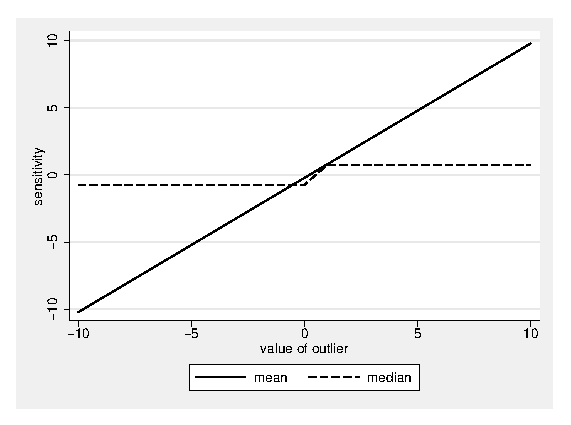
\epsfig{file=eps/2/4}
    \caption{Standardized sensitivity curves of the mean and the median for a sample of $n=20$ random $\mathcal{N}(0,1)$ numbers}
    \label{fig:theory:SClocation}
\end{figure}

\begin{figure}[h!]
    \centering
    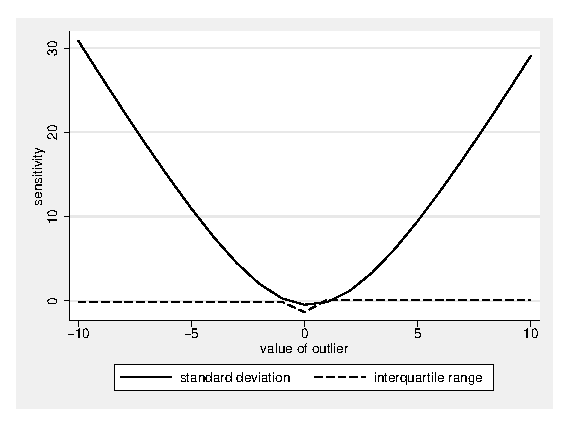
\epsfig{file=eps/2/5}
    \caption{Standardized sensitivity curves of the standard deviation and the interquartile range for a sample of $n=20$ random $\mathcal{N}(0,1)$ numbers}
    \label{fig:theory:SCscale}
\end{figure}

\index{subject}{sensitivity curve|)}

\subsubsection{The influence function}
\index{subject}{influence function|(textbf}

An intuitive way to introduce the \emph{influence function} (\stsc{IF}) of
functional $T$ at some distribution $F$ is to think of the influence function
as an asymptotic version of the \Index{sensitivity curve} of statistic $T^{(n)}=T(F^{(n)})$
when the sample size $n$ grows, so that the empirical distribution function
$F^{(n)}$ tends to the underlying population distribution function $F$ (cf.\
\citealp{hampel:1974}). More precisely, the influence function is defined as
%
\begin{align*}
    \stsc{IF}(x; T, F) 
        &= \lim_{n\rightarrow\infty} \frac{T\left(\left(1-\frac{1}{n+1}\right) F + 
            \frac{1}{n+1} \Delta_x\right) - T(F)}{\frac{1}{n+1}} \\
        &= \lim_{\varepsilon\rightarrow 0} \frac{T\left((1-\varepsilon) F + 
            \varepsilon\Delta_x\right) - T(F)}{\varepsilon}
\end{align*}
%
where $\Delta_x$ is a probability distribution with all its mass at point
$x$. That is, the influence function measures the effect on $T$ of a
perturbation of $F$ obtained by adding a small probability mass at point $x$. The expression of
$\stsc{IF}(x;T,F)$ can be found for most functionals $T$. In
chapter~\ref{chap:stats} we will provide the influence functions
of various measures of location, scale, skewness and tails heaviness.

\index{subject}{influence function|)}

\subsubsection{The gross-error sensitivity}
\index{subject}{gross-error sensitivity|(textbf}

Since $\stsc{IF}(x; T, F)$ quantifies the influence on $T$ of an infinitesimal
contamination of the distribution $F$ at point $x$, it is a \emph{local}
measure of robustness. It may be completed by a more global measure, the
\emph{gross-error sensitivity} of $T$ at distribution $F$, defined as
\[
    \gamma^*(T, F) = \sup_x \left| \stsc{IF}(x; T, F) \right|.
\]
$\gamma^*(T, F)$ evaluates to the biggest influence an outlier can have on
the functional $T$. With respect to robustness it is desirable to use an
estimator that is associated with a functional $T$ for which $\gamma^*(T, F)$ 
is finite (that is, for which the influence function is bounded).

\index{subject}{gross-error sensitivity|)}

\subsubsection{The local-shift sensitivity}
\index{subject}{local-shift sensitivity|(textbf}

The local-shift sensitivity is another tool related to the influence function;
it aims at measuring the effect of “wiggling” an observation, that is, of a
small perturbation as opposed to gross error. This is useful to asses the
effects of rounding, grouping, or other local inaccuracies.

Jumps in the \Index{influence function} (\stsc{IF}) indicate that a small
fluctuation of the value of $x$ can cause an abrupt change in the estimate.
Hence, from the perspective of robustness, we prefer a continuous \stsc{IF}
with an appropriately bounded derivative (wherever the derivative exists). 
To appreciate this kind of characteristic
of the \textit{IF}, we may determine the \emph{local-shift sensitivity}:
\[
    \lambda^*(T, F) = \sup_{x\neq y} \frac{|\stsc{IF}(y; T, F) - \stsc{IF}(x; T, F)|}
                                          {|y - x|}\ \cdot
\]

\index{subject}{local-shift sensitivity|)}

\subsubsection{The asymptotic variance of an estimator}
\index{subject}{asymptotic variance|(textbf}

The \Index{influence function} may also be used as a heuristic tool to determine the
asymptotic variance of the estimators. Indeed, under some regularity conditions
for the functional $T$, we have, under $F$,                                    
\[
    \sqrt{n}\left(T(F^{(n)}) - T(F)\right) \stackrel{d}\rightarrow \mathcal{N}\left(0, \stsc{ASV}(T, F)\right)
\]
where
\begin{equation}\label{eq:ASV}
    \stsc{ASV}(T, F) = \int_{-\infty}^\infty \stsc{IF}(x; T, F)^2 \dif F(x)
\end{equation}
(cf.\ \citealp[p. 85 and 226]{hampel:etal:1986}). Consequently, under $F$, the
interval
\[
    \left[ T(F^{(n)}) - z_{1-\alpha/2} \sqrt{\frac{\stsc{ASV}(T, F)}{n}}\ ,\  
           T(F^{(n)}) + z_{1-\alpha/2} \sqrt{\frac{\stsc{ASV}(T, F)}{n}}\right]
\]
where $z_{1-\alpha/2}$ is the quantile of order $(1-\alpha/2)$ of the ${\cal
N}(0,1)$ distribution, provides an asymptotic confidence interval for the
parameter $T(F)$, at a confidence level of $(1-\alpha)$. 

If the distribution $F$, and hence the asymptotic variance $\stsc{ASV}(T, F)$,
are not known, it is possible to obtain an approximate estimate of the confidence
interval for $T(F)$ by evaluating $\stsc{ASV}(T, F)$ at the empirical distribution 
$F^{(n)}$ (see, e.g., \citealp[79-81]{staudte:sheather:1990}). That is, an 
approximate estimate of the asymptotic variance of $T(F)$ can be obtained as
\[
    \widehat{\stsc{ASV}}(T, F) = E_{F^{(n)}}\left[\stsc{IF}\left(x; T, F^{(n)}\right)^2\right] = 
    \frac{1}{n} \sum_{i=1}^n \stsc{IF}\left(x_i; T, F^{(n)}\right)^2
\]
where $\stsc{IF}(X_i; T, F^{(n)})$ is the value of the “empirical” influence
function evaluated at observation $x_i$, in which all unknown quantities are
replaced by sample estimates. In an i.i.d.\ sample, dividing by $n$ and taking
the square root provides the \emph{influence function estimate} of the standard
error \citep[79]{staudte:sheather:1990} that can then be used to perform
significance tests or to construct confidence intervals. A similar approach can
be followed in complex samples that involve unequal sampling probabilities,
clustering, and stratification. Since the expectation of an influence function
is equal to zero, a straight forward approach is to compute the values of
$\stsc{IF}(X_i; T, F^{(n)})$ and then apply a standard mean estimator such as
\rref{mean} (possibly with the \stcmd{svy} prefix; see \rref{svy estimation})
to obtain the sampling variance. The procedure can also be applied to the
influence functions of several estimators or across several subpopulations
simultaneously to obtain the full variance-covariance matrix of the estimates.

A further possibility to obtain a confidence interval for $T(F)$ is by an by an
appropriate \Index{resampling} method such as, e.g., non-parametric bootstrap
(\citealp{davisonhinkley97}; see \rref{bootstrap}). Standard errors and
confidence intervals obtained by resampling methods my exhibit better
small-sample properties than estimates obtained by the influence function
approach.

\index{subject}{asymptotic variance|)}

\subsection{The breakdown point}
\index{subject}{breakdown point|(textbf}
\label{subsec:theory:BP}

The \Index{sensitivity curve} shows how an estimator reacts to the introduction
of one single outlier. Some estimators cannot resist even against a
single outlier. As we have seen, this is the case for the mean and the
\Index{standard deviation}. Other estimators, such as the \Index{median} and
the \Index{interquartile range}, are robust against this type of
contamination because their \Index{sensitivity curve} (\stsc{SC}) is
bounded. Possibly, however, the number of outliers in a sample is so large that
even estimators with a bounded \stsc{SC} can no longer resist their effect.
Hence, to evaluate different estimators, it is important to know what the
amount of contamination is an estimator can tolerate. The
\emph{breakdown point} is a measure for such \emph{resistance} of an estimator.
It quantifies, roughly, the smallest amount of contamination in the
sample that may cause the estimator to take on arbitrary values. Its definition
is as follows.

\subsubsection{The finite-sample breakdown point}
\index{subject}{breakdown point!finite-sample|(textbf}

The breakdown point $\epsilon^{*(n)}(T^{(n)}; \mathcal{X}^{(n)})$ of the statistic
$T^{(n)} = T^{(n)}(x_1, \dots, x_n) = T(F^{(n)})$ at the sample $\mathcal{X}^{(n)}
= \{x_1, \dots, x_n\}$ refers to the smallest proportion of observations
in $\mathcal{X}^{(n)}$ that need to be replaced to cause the value of the
statistic to be arbitrarily large or small, and hence, to make the statistic
worthless or meaningless. Note that, typically, $\epsilon^{*(n)}$ is
independent of $x_1, \dots, x_n$.

More formally, for a univariate location estimator $T^{(n)}$, which breaks down
if its absolute value becomes arbitrarily large, we may define the (finite-sample)
breakdown point as follows (see \citealp{hampel:stahel:1982};
\citealp{donoho:huber:1983}). In a given sample $\mathcal{X}^{(n)} = \{x_1,
\dots, x_n\}$, let us replace $m$ data points $x_{i_1}, \dots, x_{i_{m}}$
by arbitrary values $y_1, \dots, y_{m}$; let us call the new data set       
$\mathcal{Z}^{(n)} = \{z_1, \dots, z_n\}$. Then the \emph{(finite-sample
gross-error) breakdown point} of the estimator is
\[
    \epsilon^{*(n)}(T^{(n)}; \mathcal{X}^{(n)}) 
    = \min \left\{\left. \frac{m}{n}\right| \max_{i_i, \dots, i_{m}} \sup_{y_1, \dots, y_{m}} 
      \left|T^{(n)}(z_1, \dots, z_n)\right| =\infty \right\}.
\]

Following the same idea, we will say that a scale estimator breaks down if it
takes on a value that is arbitrarily large (scale explosion) or close to zero
(scale implosion). Furthermore, a \Index{skewness} or \Index{kurtosis}
estimator, which is bounded by $[-1, 1]$, breaks down if the absolute value of
the estimate attains the value of 1.

\begin{stexample}
If the $i$th observation among $x_1, \dots, x_n$ goes to infinity, the \Index{mean}
$\mu^{(n)}$ and the \Index{standard deviation} $\sigma^{(n)}$ go to infinity as well. This
means that the finite-sample breakdown point of these two statistics is $1/n$.
In contrast, the finite-sample breakdown point of the \Index{median} $Q_{0.5}^{(n)}$ is
$\frac{(n/2)}{n}$ if $n$ is even and $\frac{(n+1)/2}{n}$ if $n$ is odd. That is,
half the data or a bit more must be replaced to make the \Index{median} take on arbitrary
values. The finite-sample breakdown point of the \Index{interquartile range}
$\stsc{IQR}^{(n)}$ is equal to $\frac{\lfloor n/4 \rfloor + 1}{n}$, where
$\lfloor n/4 \rfloor $ denotes the integer part of $n/4$. That is, a bit more than 
one fourth of the data needs to be replaced to make the \stsc{IQR} break down.
\end{stexample}

\index{subject}{breakdown point!finite-sample|)}


\subsubsection{The asymptotic breakdown point}
\index{subject}{breakdown point!asymptotic|(textbf}

The \emph{asymptotic breakdown point} $\epsilon^*(T, F)$ of the functional
$T$ under the distribution $F$ is defined as
\[
    \epsilon^*(T, F) = \lim_{n\rightarrow\infty} \epsilon^{*(n)}(T^{(n)}; \mathcal{X}^{(n)})
\]
with the $x_i$'s sampled from $F$ (cf.\ \citealp{hampel:1971}).

\index{subject}{breakdown point!asymptotic|)}
\index{subject}{breakdown point|)}

\alert{[I would delete subsections "2.2.3 Gaussian efficiency" and "2.2.4
Aspects of interpretation". These subsections do not refer to robustness in the
presence of outliers; there are related with classical properties of
estimators, presented previously. I have modified the subsection "Summary" in
order to take into account some ideas that play an important role in the choice
of a robust estimator.]}

%\subsection{Gaussian efficiency}
%\index{subject}{Gaussian efficiency|(textbf}

%In general, if $F$ it is known, the ML-estimator for that $F$ is most efficient
%(see above). Furthermore, for $F$ equal Gaussian, the mean is the ML-estimator
%and hence most efficient. Robust estimators should not only be efficient with
%respect to Gaussian, but for a wide variety of distributions. However, Gaussian
%efficiency is also important if robust estimators are viewed as competitors of
%standard estimators. Hence it is often good to know (relative) Gaussian
%efficiency and then complement this with relative efficiencies for other
%distributions.

%\alert{[Give formal definitions etc. This is not only about Gaussian
%efficiency. For example, the mean has high variance under fat-tails
%distributions; robust estimators can have better efficiency in such cases...]}

%\index{subject}{Gaussian efficiency|)}

%\subsection{Aspects of Interpretation}

%\alert{[What about asymmetric distributions and interpretation? (e.g.
%Median vs. Mean) Need to address such aspects. The point is that robust
%estimators often estimate something that is conceptually different than the
%nonrobust counterpart (or something where robust and nonrobust counterparts
%coincide only in special situations, such as in a symmetric distribution or in
%a normal distribution).]}

\subsection{Summary}

How do we choose a good robust estimator? We are clearly interested in estimators with

\begin{enumerate}
    \item a \emph{bounded} (low \Index{gross-error sensitivity})
    and \emph{smooth} (low \Index{local-shift sensitivity}) \emph{\Index{influence function}} 

    \item and a \emph{high \Index{breakdown point}}.
\end{enumerate}

Moreover, we are looking for robust estimators that enjoy good efficiency for
a wide variety of distributions. In general, however, compromises between
robustness and efficiency must be made to achieve good overall performance, as
is shown in the following section.

Finally, we also wish to use asymptotically and Fisher consistent robust
estimators, whose rate of convergence is not smaller than the usual rate of
convergence---equal to $\sqrt{n}$---in the parametric context.


\endinput
